\section{Further results}
\label{app:modelll}
In Figs.~\ref{fig:bounds_ann}, \ref{fig:bounds_decay}, \ref{fig:all_channels_ann}, \ref{fig:all_channels_dec}, \ref{fig:bounds2}, \ref{fig:bounds3}, we show additional results on the constraints for the DM annihilation cross-section and the decay lifetime, exploring various annihilation and decay channels, as well as different observation times. We also provide further comparisons with existing bounds from the literature. 

\begin{figure}[t!]
    \centering
    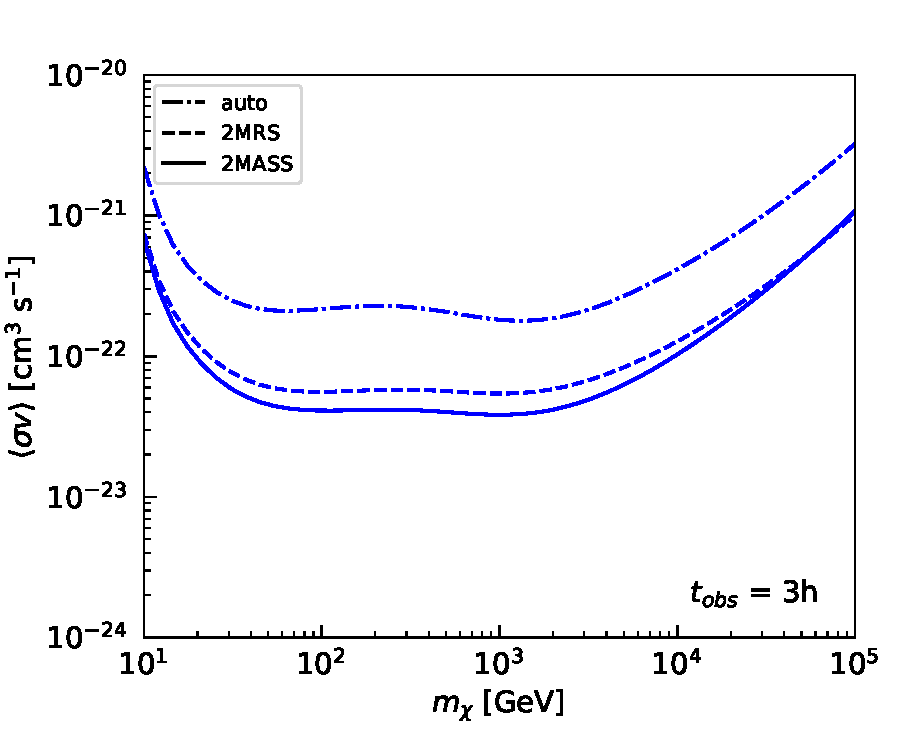
\includegraphics[width=0.45\textwidth]{figures/new_analysis/bounds/sigmav_bound_3h_b.pdf}
    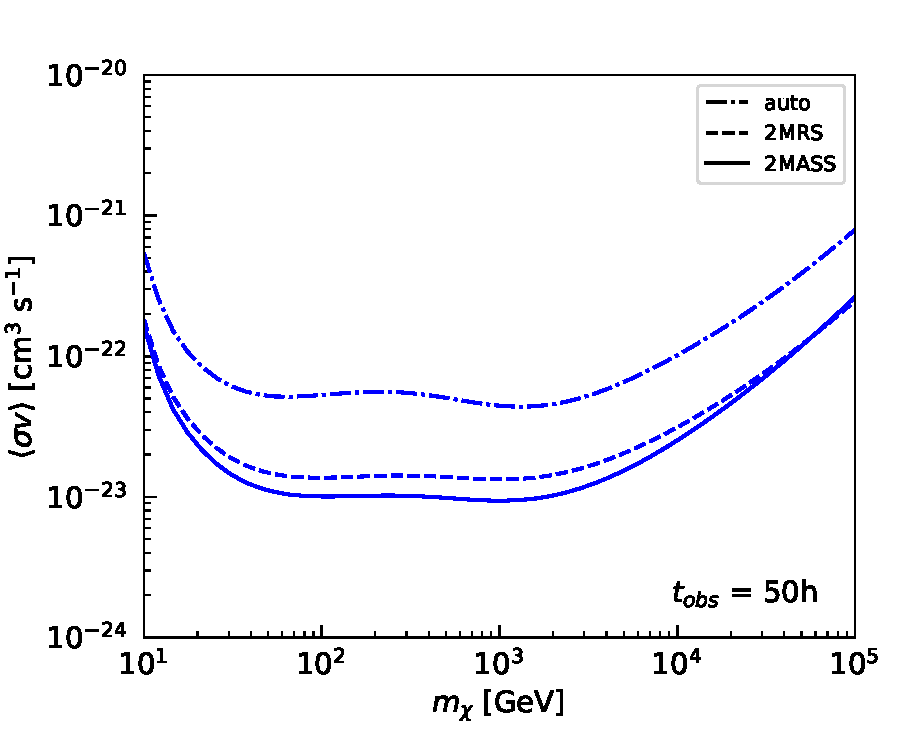
\includegraphics[width=0.45\textwidth]{figures/new_analysis/bounds/sigmav_bound_50h_b.pdf}
    \caption{Predicted upper bounds on the dark matter cross-section $\langle \sigma v \rangle$, for annihilation into $b\bar{b}$, for 3 hours (left panel) and 50 hours (right panel) of CTAO observations. The bounds are derived from $\gamma$-ray auto-correlation (dot-dashed), and cross-correlation with 2MRS (dashed lines) and 2MASS (solid) galaxy catalogs.}
    \label{fig:bounds_ann}
\end{figure}

\begin{figure}[t!]
    \centering
    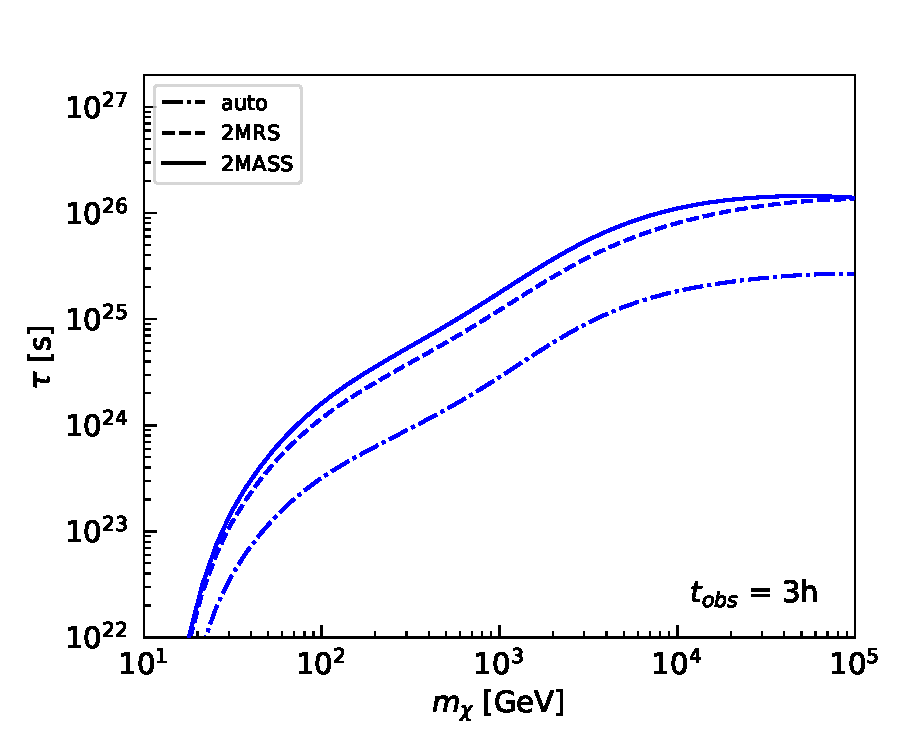
\includegraphics[width=0.45\textwidth]{figures/new_analysis/bounds/tau_bound_3h_b.pdf}
    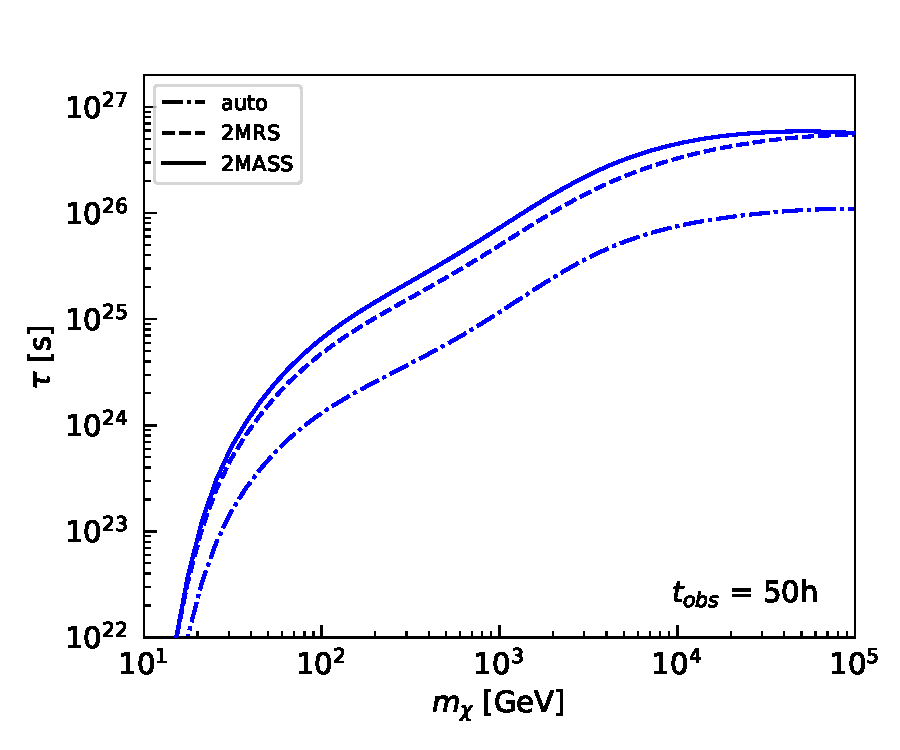
\includegraphics[width=0.45\textwidth]{figures/new_analysis/bounds/tau_bound_50h_b.pdf}
    \caption{Predicted lower bounds on the dark matter lifetime $\tau$, for decay into $b\bar{b}$, for 3 hours (left panel) and 50 hours (right panel) of CTAO observations. The bounds are derived from $\gamma$-ray auto-correlation (dot-dashed), and cross-correlation with 2MRS (dashed lines) and 2MASS (solid) galaxy catalogs.}
    \label{fig:bounds_decay}
\end{figure}

\begin{figure}[t!]
    \centering
    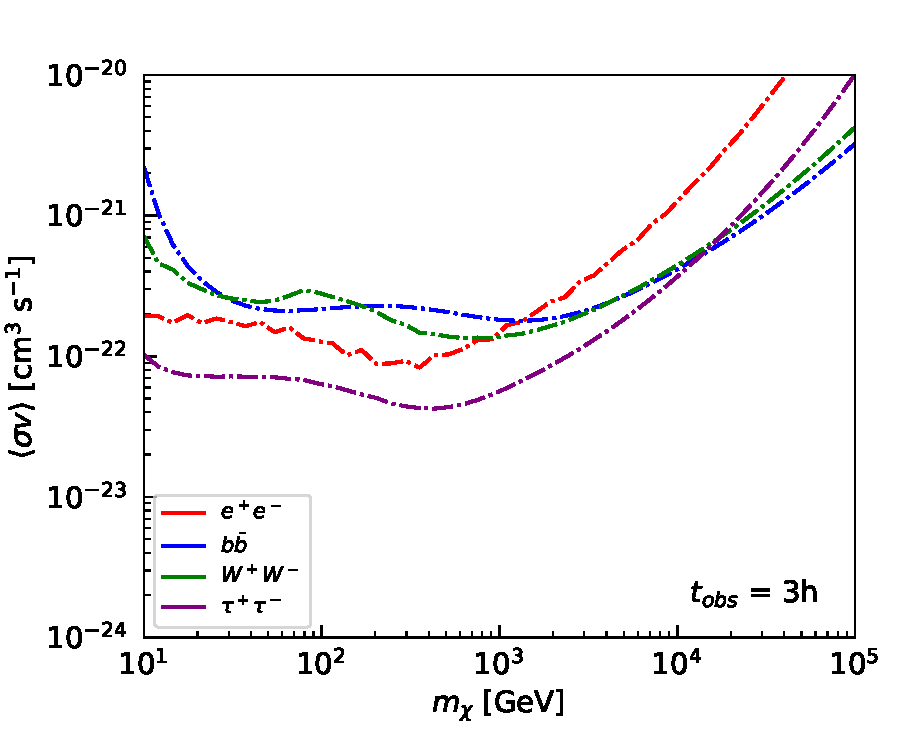
\includegraphics[width=0.45\textwidth]{figures/new_analysis/bounds/sigmav_bound_3h_e_b_W_tau_auto.pdf}
    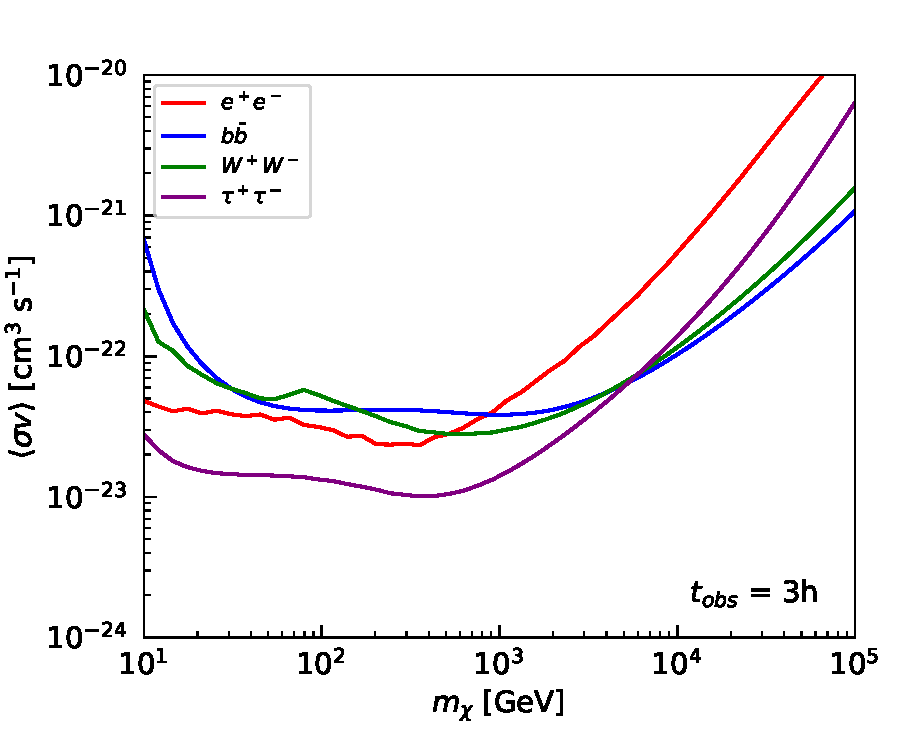
\includegraphics[width=0.45\textwidth]{figures/new_analysis/bounds/sigmav_bound_3h_e_b_W_tau_cross.pdf}
    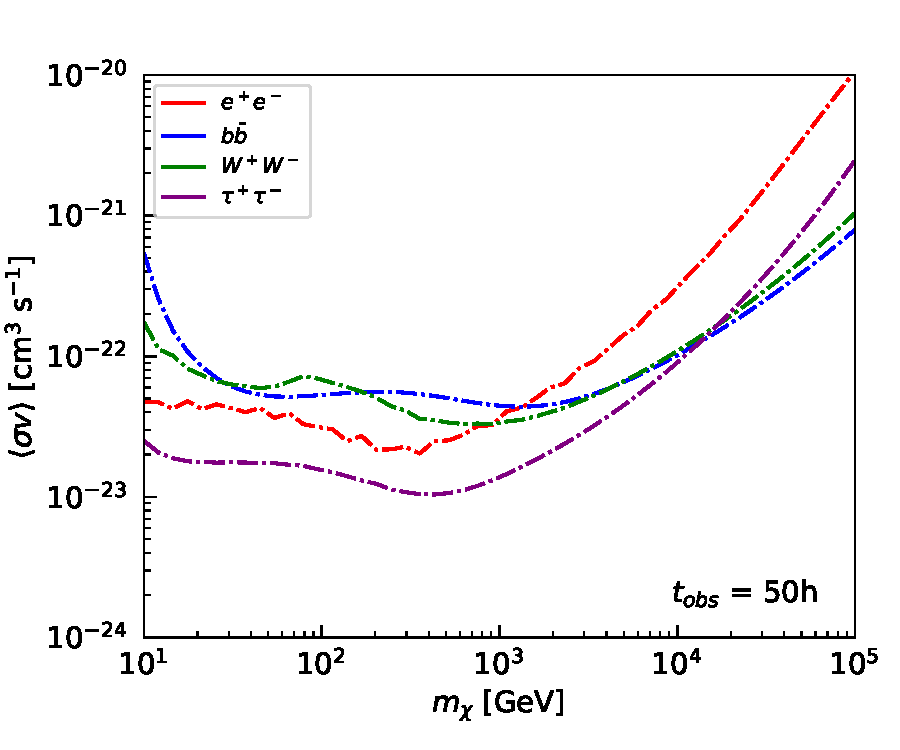
\includegraphics[width=0.45\textwidth]{figures/new_analysis/bounds/sigmav_bound_50h_e_b_W_tau_auto.pdf}
    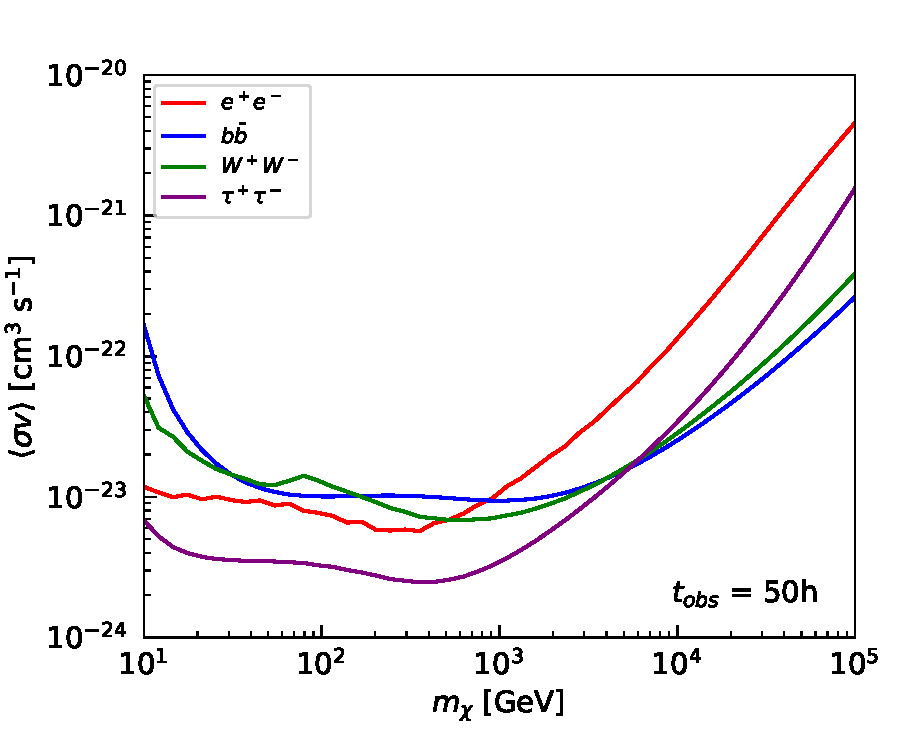
\includegraphics[width=0.45\textwidth]{figures/new_analysis/bounds/sigmav_bound_50h_e_b_W_tau_cross.pdf}
    \caption{Predicted upper bounds on the dark matter cross-section $\langle \sigma v \rangle$, for annihilation into various final states: $e^+e^-, b\bar{b}$, $W^+W^-$ and $\tau^+\tau^-$. The upper row shows results for 3 hours of observation; the lower row for 50 hours. Left panels: bounds from $\gamma$-ray auto-correlation. Right panels: bounds from cross-correlation with 2MASS galaxies (the bottom-right panel reproduces the left panel of \cref{fig:all_channels1}).}
    \label{fig:all_channels_ann}
\end{figure}


\begin{figure}[t!]
    \centering
    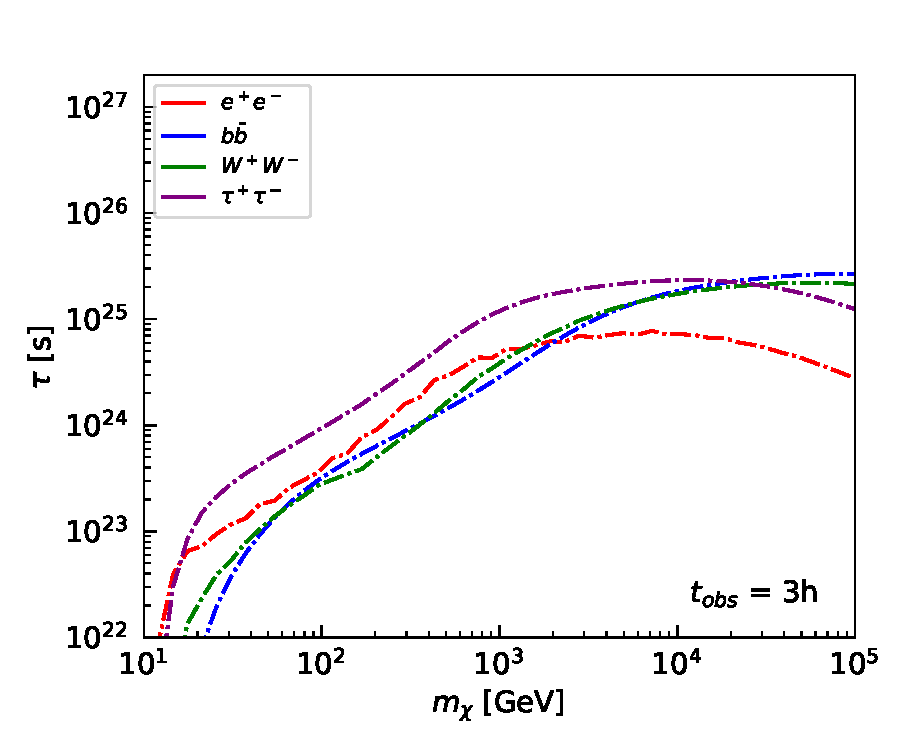
\includegraphics[width=0.45\textwidth]{figures/new_analysis/bounds/tau_bound_3h_e_b_W_tau_auto.pdf}
    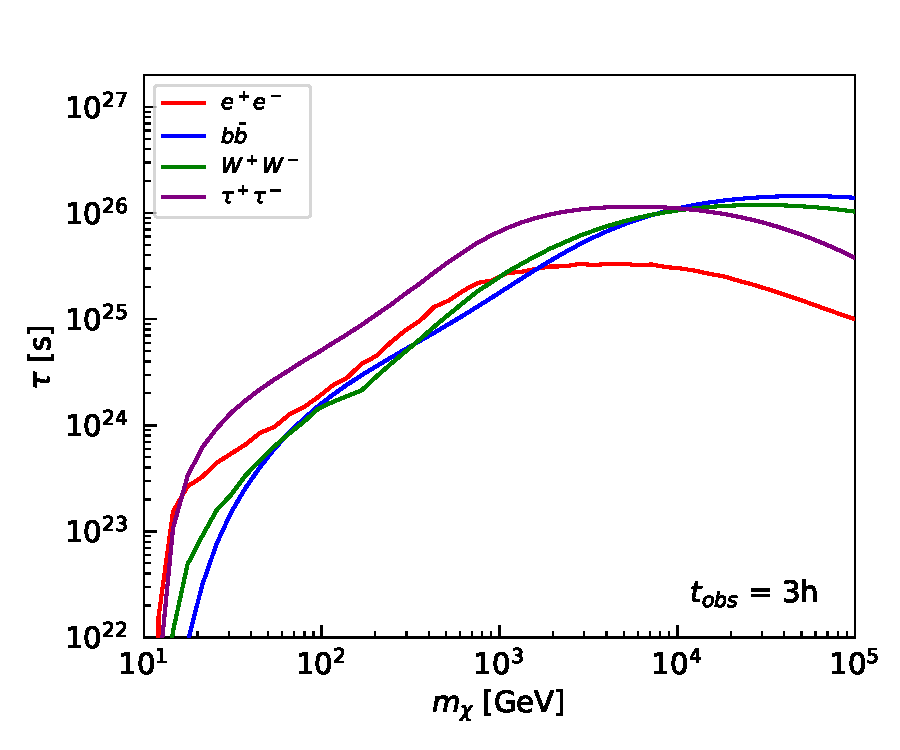
\includegraphics[width=0.45\textwidth]{figures/new_analysis/bounds/tau_bound_3h_e_b_W_tau_cross.pdf}
    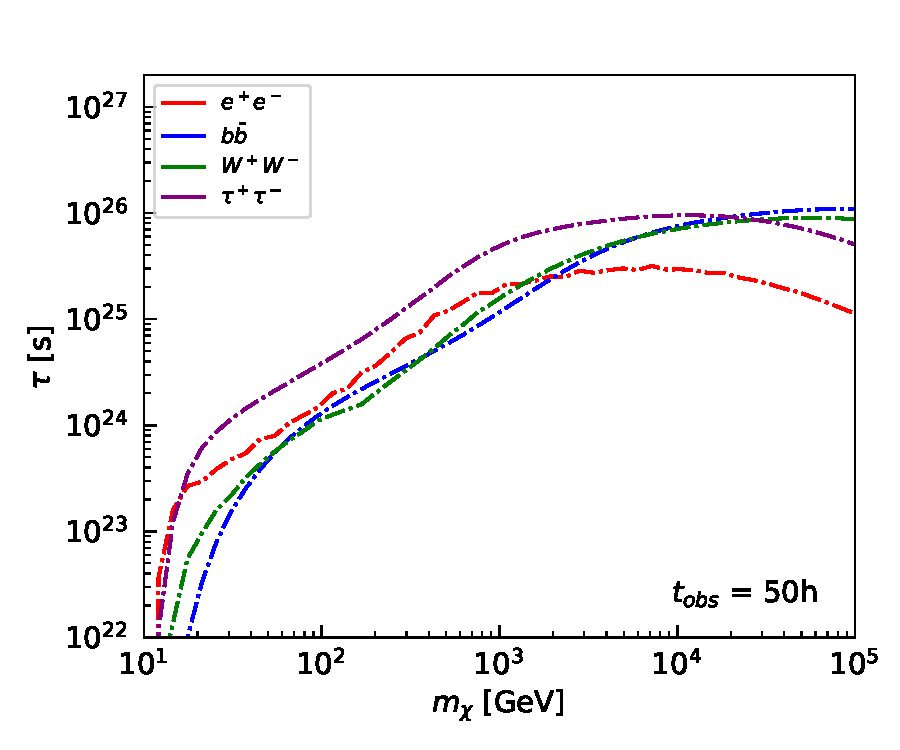
\includegraphics[width=0.45\textwidth]{figures/new_analysis/bounds/tau_bound_50h_e_b_W_tau_auto.pdf}
    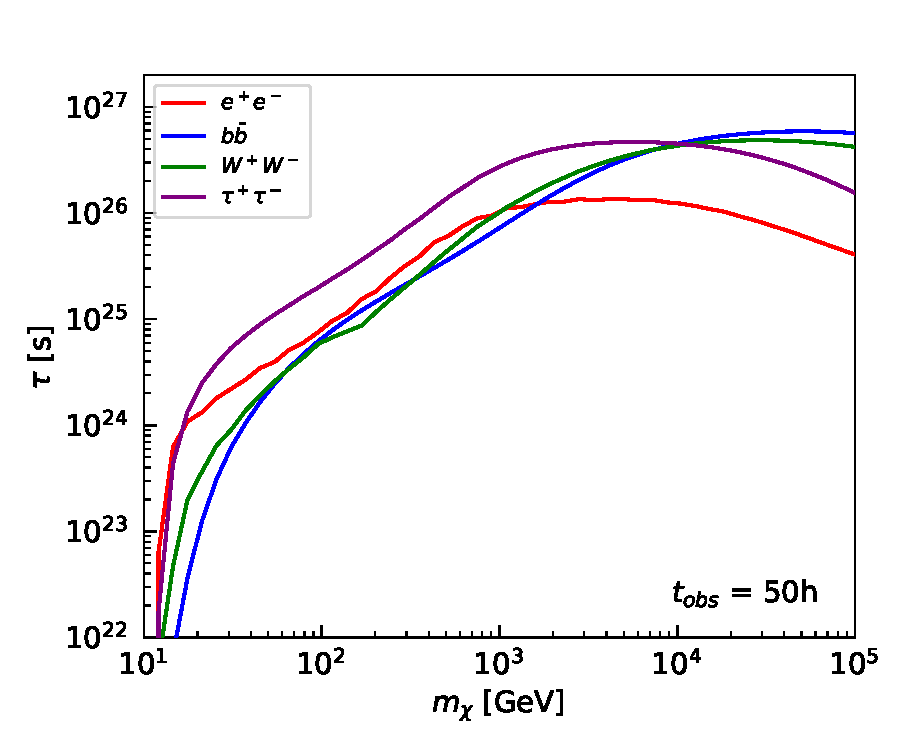
\includegraphics[width=0.45\textwidth]{figures/new_analysis/bounds/tau_bound_50h_e_b_W_tau_cross.pdf}
    \caption{Predicted lower bounds on the dark matter lifetime $\tau$, for decay into various final states: $e^+e^-, b\bar{b}$, $W^+W^-$ and $\tau^+\tau^-$. The upper row shows results for 3 hours of observation; the lower row for 50 hours. Left panels: bounds from the $\gamma$-ray auto-correlation. Right panels: bounds from cross-correlation with 2MASS galaxies (the bottom-right panel reproduces the right panel of \cref{fig:all_channels1}).}
    \label{fig:all_channels_dec}
\end{figure}

\begin{figure}[t!]
    \centering
    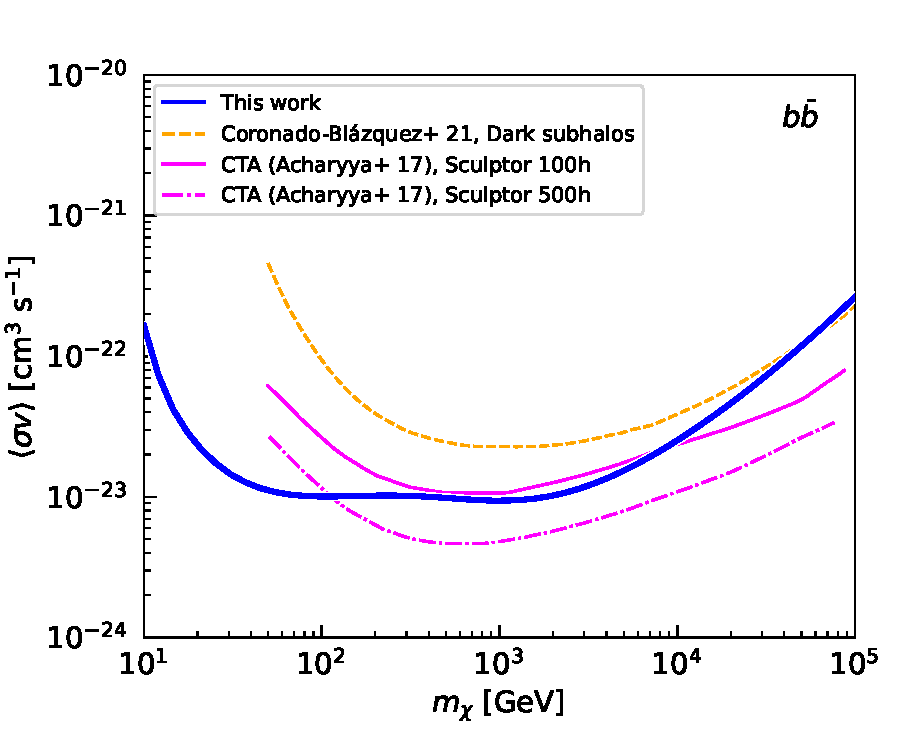
\includegraphics[width=0.45\textwidth]{figures/new_analysis/bounds/sigmav_bound_b_cross+lit-bb.pdf}
    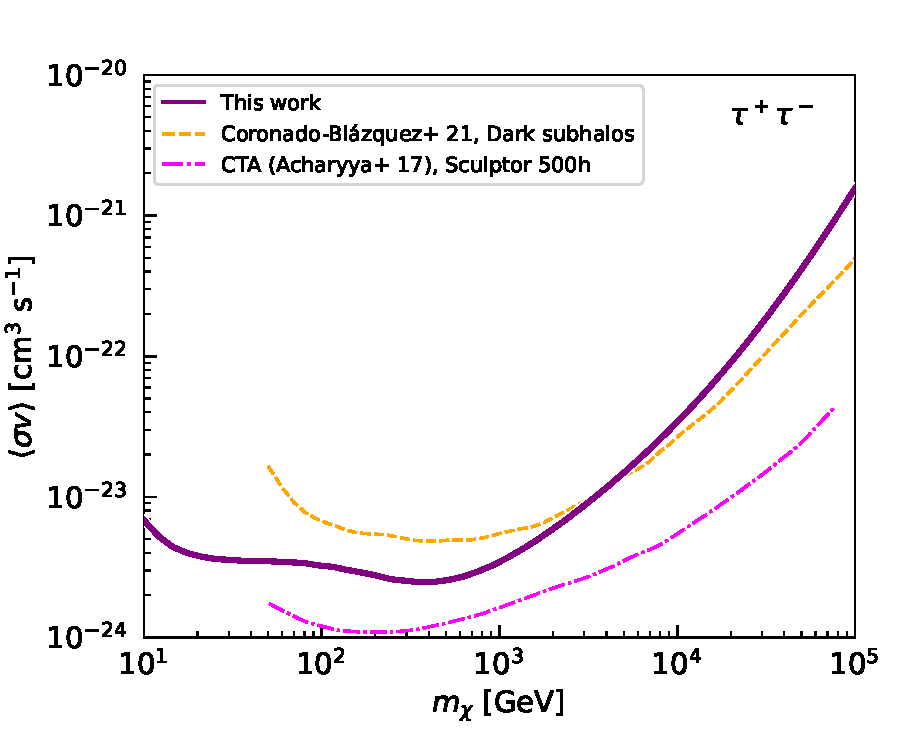
\includegraphics[width=0.45\textwidth]{figures/new_analysis/bounds/sigmav_bound_tau_cross+lit-tau.pdf}
    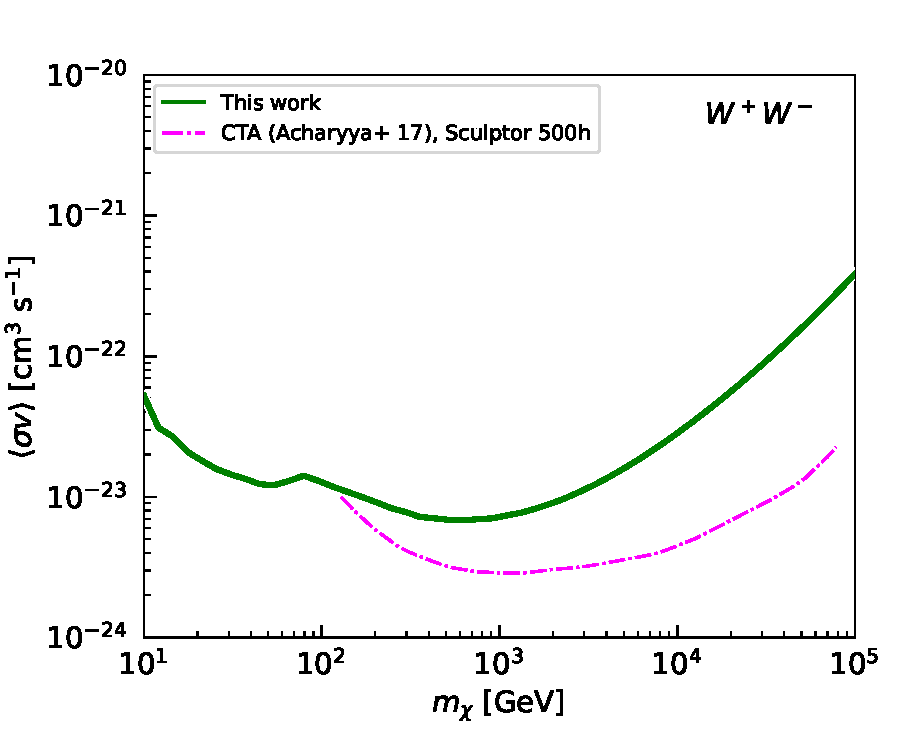
\includegraphics[width=0.45\textwidth]{figures/new_analysis/bounds/sigmav_bound_W_cross+lit-W.pdf}
    \caption{Comparison of the predicted upper bounds on the dark matter annihilation cross-section $\langle\sigma v \rangle$, with existing constraints from the literature: bounds from non-observation of dark sub-halos (dashed yellow) \cite{Coronado_Blazquez_2021}, from the Sculptor dwarf galaxy \cite{CTA_2017} with 100 hours (solid magenta) and 500 hours (dot-dashed magenta) of observations with CTAO. Three channels are displayed: $b\bar{b}$ (upper left panel), $\tau^+\tau^-$ (upper right) and the $W^+W^-$ (lower). The case for the $b\bar{b}$ channel is also shown in \cref{fig:bounds1}.}
    \label{fig:bounds2}
\end{figure}

\begin{figure}[t!]
    \centering
    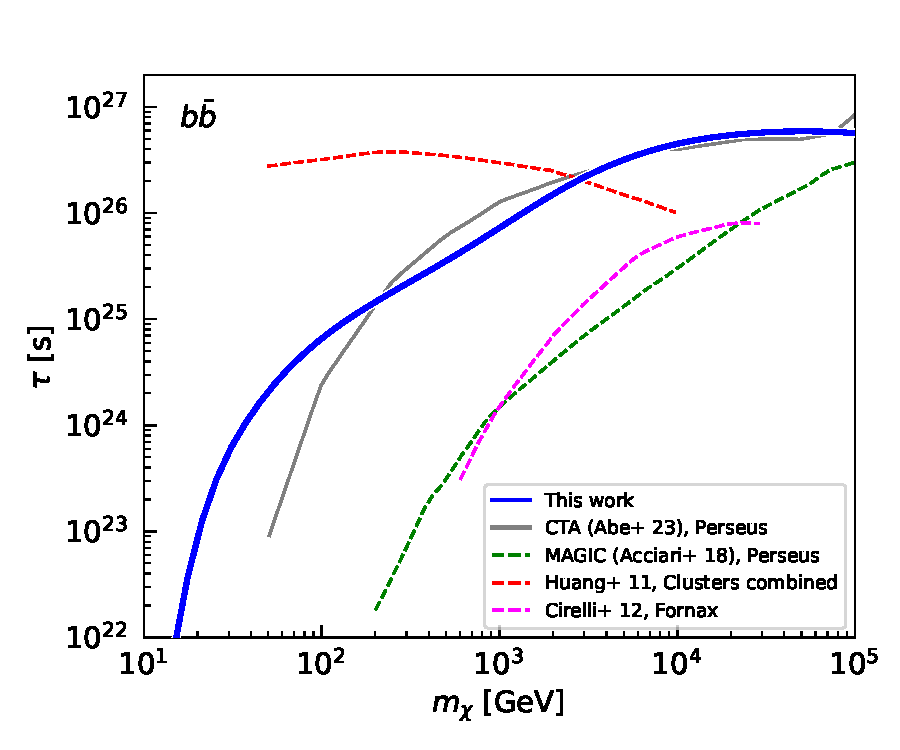
\includegraphics[width=0.45\textwidth]{figures/new_analysis/bounds/tau_bound_50h_b_cross+lit-bb.pdf}
    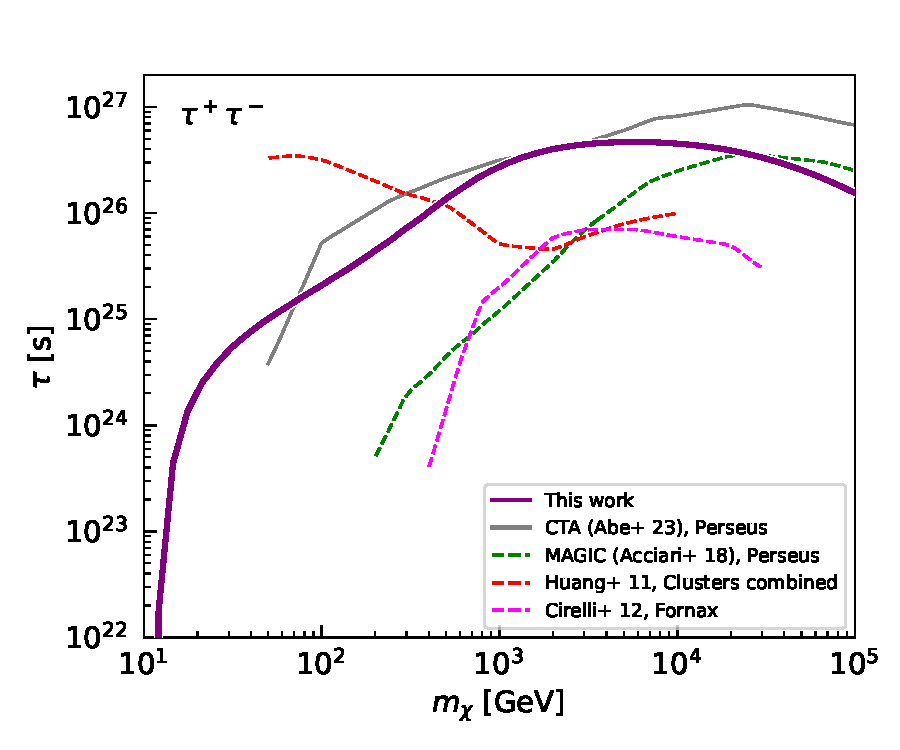
\includegraphics[width=0.45\textwidth]{figures/new_analysis/bounds/tau_bound_50h_tau_cross+lit-tau.pdf}
    \caption{Comparison of the predicted lower bounds on the DM particle lifetime $\tau$ for the $b\bar{b}$ and $\tau^+\tau^-$ decay channels, with existing constraints from the literature: limits from Perseus with CTAO \cite{CTA2023} and MAGIC \cite{MAGIC_2018}, from galaxy clusters \cite{Huang_2012}, and from Fornax \cite{Cirelli_2012}. The case for the $b\bar{b}$ channel is also shown in \cref{fig:bounds1}.}
    \label{fig:bounds3}
\end{figure}

